\frame{
  \frametitle{k-d tree\footnote{Bentley, J. L. (1975).}}
  
  
  \begin{columns}
      \begin{column}{0.5\textwidth}
          \begin{itemize}
            \item Each node is a $k$-dimensional point, each internal node splits one of the dimensions at the point.
        
            \medskip

            \item $O(\log n)$ insert, delete and search for a point, fast\footnote{subject to curse of dimensionality} range search and nearest neighbour search.
          \end{itemize}
      \end{column}
        \begin{column}{0.5\textwidth}
            \begin{center}
            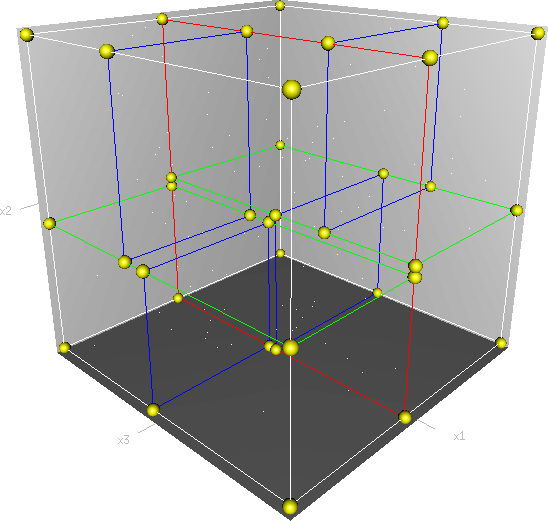
\includegraphics[scale=0.3]{slides/alphabet_trees/3dtree.png}
            \end{center}
        \end{column}
  \end{columns}
}